\documentclass[tikz,border=6pt]{standalone}
\usepackage[T1]{fontenc}
\usepackage{lmodern}
\usepackage{amsmath}
\usepackage{pgfplots}
\pgfplotsset{compat=1.18}
\usetikzlibrary{arrows.meta,positioning,fit,backgrounds,shapes.geometric,calc}
\definecolor{navy}{HTML}{16324F}
\definecolor{tealC}{HTML}{007F82}
\definecolor{amberC}{HTML}{D97706}
\definecolor{coralC}{HTML}{C2410C}
\definecolor{redC}{HTML}{DC2626}
\definecolor{mintC}{HTML}{059669}
\definecolor{slateC}{HTML}{64748B}
\definecolor{paleBg}{HTML}{F4F7FA}
\definecolor{softTeal}{HTML}{E6F4F4}
\definecolor{softNavy}{HTML}{EAF0F6}
\definecolor{softAmber}{HTML}{FEF3C7}
\begin{document}

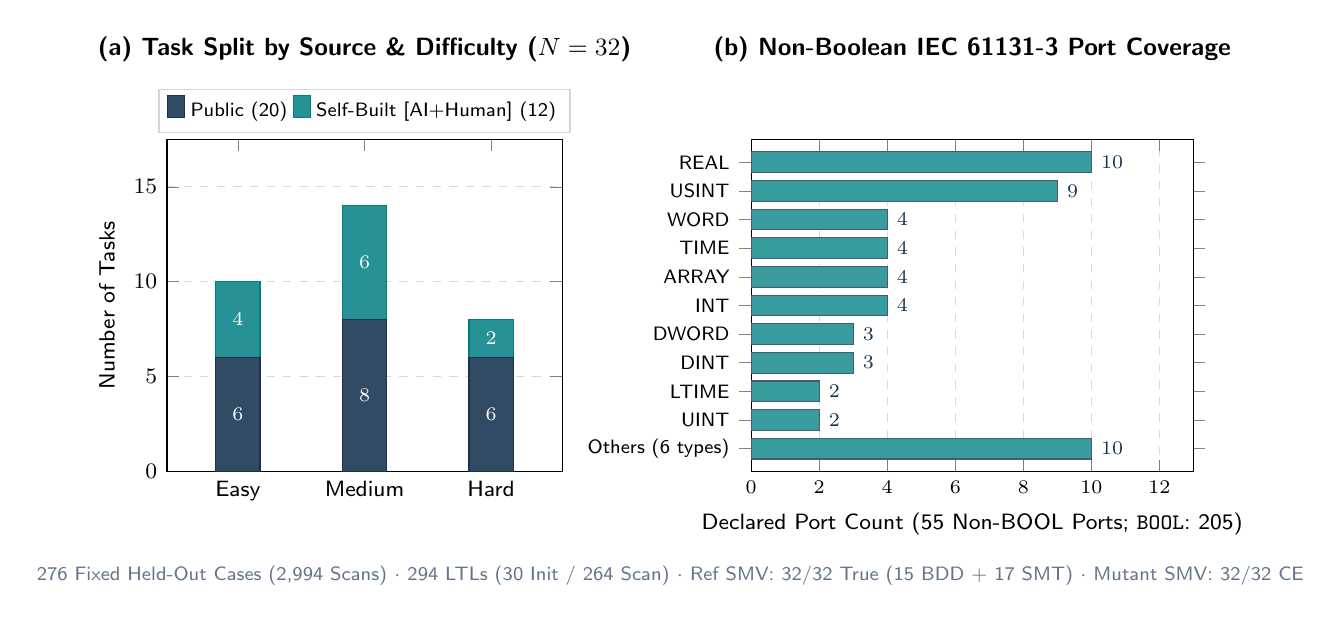
\begin{tikzpicture}
\begin{axis}[
    name=leftax,
    ybar stacked,
    bar width=16pt,
    width=6.6cm,
    height=5.8cm,
    ymin=0, ymax=17.5,
    ylabel={\footnotesize Number of Tasks},
    symbolic x coords={Easy, Medium, Hard},
    xtick=data,
    tick label style={font=\footnotesize\sffamily},
    label style={font=\footnotesize\sffamily},
    title={\small\sffamily\bfseries (a) Task Split by Source \& Difficulty ($N=32$)},
    title style={yshift=6.5mm},
    legend style={at={(0.5,1.02)}, anchor=south, legend columns=2, font=\scriptsize\sffamily, draw=navy!20, fill=white},
    nodes near coords,
    every node near coord/.append style={font=\scriptsize\sffamily\bfseries, color=white},
    ymajorgrids=true,
    grid style={dashed, gray!30},
    enlarge x limits=0.28,
]
\addplot[fill=navy!88, draw=navy] coordinates {(Easy,6) (Medium,8) (Hard,6)};
\addplot[fill=tealC!85, draw=tealC] coordinates {(Easy,4) (Medium,6) (Hard,2)};
\legend{Public (20), Self-Built [AI+Human] (12)}
\end{axis}

\begin{axis}[
    name=rightax,
    at={($(leftax.south east)+(24mm,0)$)},
    anchor=south west,
    xbar,
    bar width=7.5pt,
    width=7.2cm,
    height=5.8cm,
    xmin=0, xmax=13,
    xlabel={\footnotesize Declared Port Count (55 Non-BOOL Ports; \texttt{BOOL}: 205)},
    ytick={0,1,2,3,4,5,6,7,8,9,10},
    yticklabels={{Others (6 types)},{UINT},{LTIME},{DINT},{DWORD},{INT},{ARRAY},{TIME},{WORD},{USINT},{REAL}},
    tick label style={font=\scriptsize\sffamily},
    label style={font=\footnotesize\sffamily},
    title={\small\sffamily\bfseries (b) Non-Boolean IEC 61131-3 Port Coverage},
    title style={yshift=6.5mm},
    xmajorgrids=true,
    grid style={dashed, gray!30},
    nodes near coords,
    every node near coord/.append style={font=\scriptsize\sffamily, color=navy, anchor=west},
    enlarge y limits=0.08,
]
\addplot[fill=tealC!78, draw=navy!80] coordinates {
    (10,0)
    (2,1)
    (2,2)
    (3,3)
    (3,4)
    (4,5)
    (4,6)
    (4,7)
    (4,8)
    (9,9)
    (10,10)
};
\end{axis}

\node[font=\scriptsize\sffamily, color=slateC, anchor=north, align=center] at ($(current bounding box.south)+(0,-1.5mm)$)
  {276 Fixed Held-Out Cases (2,994 Scans) $\cdot$ 294 LTLs (30 Init / 264 Scan) $\cdot$ Ref SMV: 32/32 True (15 BDD + 17 SMT) $\cdot$ Mutant SMV: 32/32 CE};
\end{tikzpicture}
\end{document}
